% Das Buch ist lizenziert unter der Creative-Commons-Lizenz
% "Namensnennung - Weitergabe unter gleichen Bedingungen 4.0 International (CC BY-SA 4.0)"
% https://creativecommons.org/licenses/by-sa/4.0/deed.de

\chapter{Zusammengesetzte Daten}
\label{cha:zusammengesetzte-daten}

Viele Informationen, die in Programmen repräsentiert werden, haben
mehrere Bestandteilen:
%
\begin{itemize}
\item Ein Festessen besteht aus Vorspeise, Hauptgang und Nachspeise.
\item Eine Uhrzeit besteht aus Stunden und Minuten.
\item Eine Tür besteht aus Türblatt und Türgriff.
\end{itemize}
%
Es werden also mehrere Dinge zu einem \textit{zusammengesetzt}.
Eine andere Betrachtungsweise ist, dass ein einzelnes
Ding \textit{mehrere Eigenschaften} hat:
%
\begin{itemize}
\item Ein Filzstift hat Dicke und Farbe.
\item Eine Katze hat Alter und Geschlecht.
\item Ein Lautsprecher hat Minimal- und Maximalfrequenz.
\end{itemize}
%
Um solche Informationen abzubilden, führen wir in diesem Kapitel eine neue Art
Daten ein, die \textit{zusammengesetzten
  Daten}\index{zusammengesetzten Daten}.

\section{Computer konfigurieren}
\label{sec:computer-konfigurieren}

\mentioncode{zusammengesetzte-daten/computer.rkt}
%
Viele Computergeschäfte erlauben, bestimmte Komponenten
eines neues Computers auszuwählen, zum Beispiel Prozessor,
Festplatte und Größe des RAM"=Hauptspeichers:
%
\begin{center}
  \medskip
  \includegraphics[height=0.25\textheight]{zusammengesetzte-daten/computer}
  \medskip
\end{center}
%
Anders gesagt, ein Computer\index{Computer} \emph{besteht aus}:
%
\begin{itemize}
\item Prozessor
\item RAM
\item Festplatte
\end{itemize}
%
Natürlich besteht ein Computer auch noch aus anderen Teilen, die
aber (zumindest in diesem Beispiel) immer gleich oder irrelevant sind.
In einer Bestellung müssen also nur diese drei Bestandteile
enthalten sein.  Wir nehmen an, dass es beim Prozessor nur auf den Namen
("<Athlon">, "<Xeon">, "<Cell">, \ldots) ankommt, beim RAM nur auf die
Größe in Gigabyte, und auch bei der Festplatte nur auf die Größe in
Gigabyte.

Wir können daraus eine amtliche Datendefinition machen:
%
\begin{lstlisting}
; Ein Computer besteht aus:
; - Prozessor
; - Hauptspeicher-Kapazität in Gbyte
; - Festplatten-Kapazität in Gbyte
\end{lstlisting}
%
Wichtig ist hier die Formulierung "<besteht aus">, die auf
zusammengesetzte Daten hindeutet.  Die Daten, die aus so einer
Datendefinition für zusammengesetzte Daten entstehen, können als
Tabelle dargestellt werden:
%
\begin{center}
  Computer\qquad
  \begin{tabular}[c]{r|l}
    \textbf{Feld} & \textbf{Komponente}\\\hline
     Prozessor & \verb|"Cell"|\\
     RAM & 8\\
    Festplatte & 250
  \end{tabular}
\end{center}
%
Diese Tabelle steht demnach für einen Computer mit Cell-Prozessor, 8
Gigabyte RAM und einer 250-Gigabyte-Festplatte.  Sie hat also mehrere
Bestandteile und ist damit zusammengesetzt.  Die Computerfirma wird
viele Computer nach diesem Schema ausliefern, bei denen allesamt
jeweils Prozessor, RAM und Festplatte in der Bestellung stehen wird.  Solche
Informationen, die alle dem gleichen Schema folgen, können also nach
"<Typ"> sortiert werden, wobei der Typ
festlegt, um was für eine Art Information es geht und aus welchen
Teilen sie zusammengesetzt ist.  In der obigen Tabelle ist das
\textit{Feld} die Allgemeinbezeichnung für ein Bestandteil, das
alle Computer haben.  Die \textit{Komponente} ist das konkrete
Bestandteil eines einzelnen Computers.

Zusammengesetzte Daten bilden die Lehrsprachen durch
sogenannte \textit{Records}\index{Records} ab.  Jeder Record gehört
zu einem bestimmten
\textit{Record-Typ\index{Record-Typ}}, der festlegt, was für eine
Sorte Information repräsentiert wird und welche Felder die Records
des Record-Typs haben.

Der Record-Typ für Computer sieht feste Felder\index{Feld}
vor ("<Prozessor">, "<RAM">, "<Festplatte">).  Ein einzelner Record
dieses Typs besteht aus Komponenten\index{Komponente}, eine pro
Feld. (In diesem Fall \lstinline{"Cell"}, $8$ und $250$.)

Record-Typen müssen in einem Programm explizit mit Hilfe einer
speziellen \textit{Record-Definition}\index{Record-Definition} definiert werden, die mit
\lstinline{define-record} beginnt.  Hier ist die
Record-Definition zur Datendefinition für
Computer:\indexvariable{define-record}
%
\begin{lstlisting}
(define-record computer
  make-computer
  (computer-processor  string)
  (computer-ram        natural)
  (computer-hard-drive natural))
\end{lstlisting}
%
Diese etwas komplizierte Form erläutern wir Schritt für Schritt.  Weil sie gleich mehrere
Funktionen definiert, die mit Records zu tun haben, heißt
sie \lstinline{define-record}.  Nach
\lstinline{define-record} steht der Name der Signatur für
die Werte des Record-Typs,
\lstinline{computer}.  Diese Signatur nennen wir ab sofort die
\textit{Record-Signatur}.\index{Record-Signatur}

Als Nächstes in der Record-Definition kommt \lstinline{make-computer},
der Name einer Funktion, die für die \textit{Konstruktion} eines
Computer"=Records zuständig ist.  Analog zum Zusammenbauen eines
Computers mit Cell-Prozessor, 8 Gigabyte RAM und 250 Gigabyte
Festplatte wird der dazugehörige Record mit der Funktion
\lstinline{make-computer} folgendermaßen hergestellt:
%
\begin{lstlisting}
(make-computer "Cell" 8 250)
|\evalsto| #<record:computer "Cell" 8 250>
\end{lstlisting}
%
\lstinline{Make-computer} hat folgende Signatur:
%
\begin{lstlisting}
(: make-computer (string natural natural -> computer))
\end{lstlisting}
%
Die drei Eingaben sind der Reihe nach Prozessor, RAM und Festplatte.
\lstinline{Make-computer} macht daraus einen Wert der Sorte
\lstinline{computer} der Computer-Records.  Da \lstinline{make-computer}
einen Computer=Record "<konstruiert">, heißt die Funktion auch
\textit{Konstruktor\index{Konstruktor}}.

Mit der Schreibweise
%
\begin{lstlisting}
#<record:... ...>
\end{lstlisting}
%
werden Record-Typ und ihre Komponenten in der REPL sichtbar.

Hier sind einige Beispiele für Computer-Records, mit Kommentaren,
welche die Beziehung zwischen Daten und Information (siehe
Abschnitt~\ref{sec:information-daten} auf
Seite~\pageref{sec:information-daten}) herstellt:
%
\begin{lstlisting}
; Cell, 4 Gbyte RAM, 1000 Gbyte Festplatte
(define gamer (make-computer "Cell" 4 1000))

gamer
|\evalsto| #<record:computer "Cell" 4 1000>

; Xeon, 2 Gbyte RAM, 500 Gbyte Festplatte
(define workstation (make-computer "Xeon" 2 500))

workstation
|\evalsto| #<record:computer "Xeon" 2 500>
\end{lstlisting}
%
Umgekehrt zur Konstruktion nehmen manche Bastler aus dem Computer die
Einzelteile wieder heraus, zum Beispiel, um sie in einem anderen
Computer zu verbauen. Für dieses Herausnehmen sind die Funktionen
\lstinline{computer-processor}, \lstinline{computer-ram} und
\lstinline{computer-hard-drive} zuständig, die von der
Record-Definition definiert werden:
%
\begin{lstlisting}
(computer-processor gamer)
|\evalsto| "Cell"
(computer-ram gamer)
|\evalsto| 4
(computer-hard-drive gamer)
|\evalsto| 1000
\end{lstlisting}
%
Diese drei Funktionen heißen \textit{Selektoren\index{Selektor}}.  Sie haben
folgende Signaturen:
%
\begin{lstlisting}
(: computer-processor (computer -> string))
(: computer-ram (computer -> natural))
(: computer-hard-drive (computer -> natural))
\end{lstlisting}
%
Genau genommen sind diese Signaturen redundant: In der
Record-Definition steht ja schon, dass die Felder die Signaturen
\lstinline{string}, \lstinline{natural} und \lstinline{natural} sind.  Jeder
Selektor hat \lstinline{computer} als Eingabe und die jeweilige
Feld-Signatur als Ausgabe.  Auch die Signatur-Deklaration für den
Konstruktor ist redundant.
%
\begin{aufgabeinline}
  Wie ist der Zusammenhang zwischen der Record-Definition und der
  Signatur des Konstruktors?
\end{aufgabeinline}
%
Trotzdem ist es zumindest am Anfang hilfreich, sich die Arbeitsweise
von Konstruktor und Selektoren anhand ihrer Signaturen klarzumachen.
Wir schreiben sie darum in diesem Kapitel noch hin, danach nicht mehr.

Mit Hilfe des Konstruktors und der Selektoren können wir weitergehende
Funktionen definieren.
Für den Anfang könnte das
eine Funktion sein, die den Gesamtspeicher eines Computers berechnet,
also Hauptspeicher und Festplattenspeicher zusammen.
Eine solche Funktion müsste Kurzbeschreibung und Signatur wie folgt
haben:\indexvariable{total-memory} 
%
\begin{lstlisting}
; Gesamtspeicher berechnen
(: total-memory (computer -> natural))
\end{lstlisting}
%
Hier sind unsere Erwartungen an \lstinline{total-memory}, als Testfälle
formuliert:
%
\begin{lstlisting}
(check-expect (total-memory workstation) 502)
(check-expect (total-memory gamer) 1004)
\end{lstlisting}
% 
Das Gerüst ist wie folgt:
%
\begin{lstlisting}
(define total-memory
  (lambda (c)
    ...))
\end{lstlisting}
%
Um etwas aus dem Record zu berechnen, muss \lstinline{total-memory} (und
so gut wie jede andere Funktion auch) die Bestandteile betrachten.  Es
ist deshalb sinnvoll, die Schablone mit den Aufrufen der Selektoren zu
bestücken.
%
\begin{lstlisting}
(define total-memory
  (lambda (c)
    ... (computer-processor c) ...
    ... (computer-ram c) ...
    ... (computer-hard-drive c) ...))
\end{lstlisting}
%
Jetzt wo die Schablone fertig ist, können wir uns mit dem Inhalt der
Aufgabe beschäftigen: Der Prozessor hat nichts mit der
Speichermenge zu tun, wir können den entsprechenden Selektoraufruf
also wieder löschen:
%
\begin{lstlisting}
(define total-memory
  (lambda (c)
    ... (computer-ram c) ...
    ... (computer-hard-drive c) ...))
\end{lstlisting}
%
Der Gesamtspeicher ist die Summe der beiden Komponenten:
%
\indexvariable{total-memory}
\begin{lstlisting}
(define total-memory
  (lambda (c)
    (+ (computer-ram c)
       (computer-hard-drive c))))
\end{lstlisting}
%
\lstinline{Total-memory} ist ein Beispiel für eine Funktion, die einen
Record akzeptiert.  Umgekehrt gibt es auch Funktionen, die Records
produzieren.  Angenommen, unser Computerhändler bietet neben der
Einzelkonfiguration von Prozessor, Hauptspeicher und Festplatte einige
Standardmodelle an~-- sagen wir, ein Billigmodell, ein Modell für
Profis (was immer ein "<Profi"> sein mag) und ein Modell für
Computerspieler.  Je nachdem, welches der Modelle der Kunde auswählt,
muss die entsprechende Konfiguration zusammengesetzt werden.  Für die
Standardkonfiguration gibt es drei feste Möglichkeiten, es handelt
sich hier also um eine Aufzählung.

Für die Aufzählung machen wir erst einmal~-- nach
Konstruktionsanleitung~\ref{ka:aufzaehlung} auf
Seite~\pageref{ka:aufzaehlung}~-- eine Daten- und eine
Signatur-Definition:
%
\indexvariable{model}
\begin{lstlisting}
; Ein Modell ist eins der folgenden:
; - Billigmodell
; - Profi-Modell
; - Gamer-Modell
(define model
  (signature
   (enum "cheap" "professional" "gamer")))
\end{lstlisting}
%
Eine Funktion, die zu einer Standardkonfiguration den passenden
Computer fertigt, könnte damit folgende Kurzbeschreibung und Signatur haben:
%
\begin{lstlisting}
; Standard-Computer zusammenstellen
(: standard-computer (model -> computer))
\end{lstlisting}
%
Die Testfälle sollten alle drei Standardkonfigurationen abdecken:
%
\begin{lstlisting}
(check-expect (standard-computer "cheap")
              (make-computer "Sempron" 2 500))
(check-expect (standard-computer "professional")
              (make-computer "Xeon" 4 1000))
(check-expect (standard-computer "gamer")
              (make-computer "Quad" 4 750))
\end{lstlisting}
%
Hier ist das Gerüst:
%
\begin{lstlisting}
(define standard-computer
  (lambda (k)
    ...))
\end{lstlisting}
%
Bei der Schablone gehen wir wieder nach Konstruktionsanleitung~\ref{ka:aufzaehlung} auf
Seite~\pageref{ka:aufzaehlung} vor.
Da es sich beim Argument von \lstinline{standard-computer} um eine Fallunterscheidung~-- eine Aufzählung
mit \emph{drei} Alternativen~-- handelt, können wir die
dazu passende Schablone~-- eine Verzweigung mit \emph{drei} Zweigen~--
zum Einsatz bringen:
%
\begin{lstlisting}
(define standard-computer
  (lambda (k)
    (cond
      (... ...)
      (... ...)
      (... ...))))
\end{lstlisting}
%
Bei den Tests der Zweige müssen wir \lstinline{k} mit den Elementen der
Aufzählung vergleichen.  Da es sich um Zeichenketten handelt, nehmen
wir dazu \lstinline{string=?}:
%
\begin{lstlisting}
(define standard-computer
  (lambda (k)
    (cond
      ((string=? k "cheap") ...)
      ((string=? k "professional") ...)
      ((string=? k "gamer") ...))))
\end{lstlisting}
%
In jedem Zweig müssen wir nun dafür sorgen, dass der entsprechende
Computer hergestellt wird.  Für das Herstellen von Computer-Records
ist der Konstruktor \lstinline{make-computer} zuständig.  Dem"-entsprechend
müssen wir in jedem Zweig einen Aufruf von \lstinline{make-computer}
platzieren, jeweils mit drei Argumenten:
%
\begin{lstlisting}
(define standard-computer
  (lambda (k)
    (cond
      ((string=? k "cheap")
       (make-computer ... ... ...))
      ((string=? k "professional")
       (make-computer ... ... ...))
      ((string=? k "gamer")
       (make-computer ... ... ...)))))
\end{lstlisting}
%
Jetzt müssen wir die Argumente für die Aufrufe von
\lstinline{make-computer} zur Verfügung stellen.  Für jeden Aufruf sind
das der Prozessor, die Größe des Hauptspeichers und die
Größe der Festplatte.  Die entsprechenden Angaben können wir zum
Beispiel den Testfällen entnehmen.  Folgendes kommt dabei heraus:
%
\indexvariable{standard-computer}
\begin{lstlisting}
(define standard-computer
  (lambda (k)
    (cond
      ((string=? k "cheap")
       (make-computer "Sempron" 2 500))
      ((string=? k "professional")
       (make-computer "Xeon" 4 1000))
      ((string=? k "gamer")
       (make-computer "Quad" 4 750)))))
\end{lstlisting}
%
Fertig!

\begin{aufgabeinline}
  Schreibe eine Funktion, die einen Computer klassifiziert als
  "<fett">, "<Durchschnitt"> oder "<müde">.  Definiere die Kriterien
  dafür selbst.
\end{aufgabeinline}

\section{Zusammengesetzte Daten selbst konstruieren}

\mentioncode{zusammengesetzte-daten/wallclock-time.rkt}
%
Für ein weiteres Beispiel greifen wir auf folgenden Satz aus der
Einleitung zurück, den wir schon als Datendefinition auslegen können:
%
\begin{lstlisting}
; Eine Uhrzeit besteht aus Stunde und Minute.
\end{lstlisting}
%
Für die Entwicklung der dazu passenden Record-Definition müssen wir
uns einen Namen für den Record-Typ ausdenken.  Dann können wir bereits
ein karges Gerüst hinschreiben:\indexvariable{wallclock-time}
%
\begin{lstlisting}
(define-record wallclock-time
  make-wallclock-time
  ...)
\end{lstlisting}
%
Als Nächstes müssen wir festlegen, \emph{wie viele} Bestandteile die
Records haben sollen.  In diesem Fall ("<Stunde und Minute">) sind es
zwei.  Wir können das Gerüst der Record-Definition
entsprechend um zwei Felder erweitern:
%
\begin{lstlisting}
(define-record wallclock-time
  make-wallclock-time
  (... ...)
  (... ...))
\end{lstlisting}
%
Auf die Anzahl der Bestandteile zu achten, hilft uns dabei, 
Mantra~\ref{mantra:schreib} auf Seite~\pageref{mantra:schreib}
umzusetzen:

\mantraschreib*

\noindent Als Nächstes kommen die Namen der Selektoren.  Dabei befolgen wir eine
Konvention, die Selektoren alle mit \lstinline{wallclock-time-} anfangen
zu lassen.  Bei der Benennung des Konstruktor haben wir ebenfalls
eine Konvention angewendet, dessen Name sich aus \lstinline{make-} und
dem Namen des Record-Typs ergibt.  Also:
%
\begin{lstlisting}
(define-record wallclock-time
  make-wallclock-time
  (wallclock-time-hour   ...)
  (wallclock-time-minute ...))
\end{lstlisting}
%
Dass wir die Selektoren untereinander schreiben, dient lediglich der
Übersichtlichkeit, ist also ebenfalls eine Konvention.

Es fehlen noch
die Signaturen bei \lstinline{wallclock-time-hour} und
\lstinline{wallclock-time-minute}.  Nicht nur die: Wir brauchen
überhaupt erstmal Datendefinitionen für die beiden Felder.
%
\begin{lstlisting}
; Eine Stunde ist eine ganze Zahl zwischen 0 und 23.
; Eine Minute ist eine ganze Zahl zwischen 0 und 59.
\end{lstlisting}
%
Da es um ganze Zahlen ab 0 geht, könnten wir \lstinline{natural}
verwenden, präziser ist es aber, wenn wir \lstinline{integer-from-to}
aus Abschnitt~\ref{function:integer-from-to} auf
Seite~\pageref{function:integer-from-to} benutzen und eigene
Signatur-Definitionen einführen:
%
\indexvariable{hour}
\indexvariable{minute}
\begin{lstlisting}
; Eine Stunde ist eine ganze Zahl zwischen 0 und 23.
(define hour (signature (integer-from-to 0 23)))
; Eine Minute ist eine ganze Zahl zwischen 0 und 59.
(define minute (signature (integer-from-to 0 59)))
\end{lstlisting}
%
Diese Signaturen können wir jetzt in der Record-Definition für
\lstinline{wallclock-time} verwenden:
%
\indexvariable{wallclock-time}
\begin{lstlisting}
(define-record wallclock-time
  make-wallclock-time
  (wallclock-time-hour   hour)
  (wallclock-time-minute minute))
\end{lstlisting}
%
Wir schreiben die Signaturen der definierten Funktionen aus.  Diese
ergeben sich direkt aus der Record-Definition:
%
\begin{lstlisting}
(: make-wallclock-time (hour minute -> wallclock-time))
(: wallclock-time-hour (wallclock-time -> hour))
(: wallclock-time-minute (wallclock-time -> minute))
\end{lstlisting}
%
Der Konstruktor akzeptiert für jedes Feld ein Argument~-- entsprechend
stehen die Signaturen der Felder vor dem Pfeil.  Heraus kommt beim
Konstruktor immer ein Record, da steht also der Name des Record-Typs.

\begin{feature}{\lstinline{define-record} (einfach)}{scheme:define-record-simple}
Eine Record-Definition\index{Record-Definition}\indexvariable{define-record}
hat folgende allgemeine Gestalt:\label{def:define-record}
%
\begin{lstlisting}
(define-record |\(t\)|
  |\(c\)|
  (|\(\mathit{sel}\sb{1}\)| |\(\mathit{sig}\sb{1}\)|)
  |\(\ldots\)|
  (|\(\mathit{sel}\sb{n}\)| |\(\mathit{sig}\sb{n}\)|))
\end{lstlisting}
%
Diese Form definiert einen Record-Typ mit $n$ Feldern.
Dabei sind $t$, $c$, $\mathit{sel}_1 \ldots \mathit{sel}_n$ allesamt Variablen, für die
\lstinline{define-record} Definitionen anlegt:
%
\begin{itemize}
\item $t$ ist der Name der Record-Signatur.
\item $c$ ist der Name des Konstruktors, den
  \lstinline{define-record} anlegt.  Der Konstruktor hat 
  folgende Signatur:
%  
\begin{lstlisting}
(: $c$ ($\mathit{sig}\sb{1}$ $\ldots$ $\mathit{sig}\sb{n}$ -> $t$))
\end{lstlisting}
\item $\mathit{Sel}_1, \ldots, \mathit{sel}_n$ sind die Namen der Selektoren für die Felder
  des Record-Typs.  Der Selektor $s_i$ hat folgende Signatur:
% 
\begin{lstlisting}
(: $\mathit{sel}\sb{i}$ ($t$ -> $\mathit{sig}\sb{i}$))
\end{lstlisting}
\end{itemize}
%
\end{feature}

Bei den Selektoren ist es umgekehrt: Da steht immer die Record-Signatur
vorn (sie akzeptieren ja jeweils einen Record) und nach dem Pfeil
steht die Signatur des jeweiligen Feldes.

Abbildung~\ref{scheme:define-record-simple} fasst die Form
von Record-Definitionen zusammen.

Hier sind drei Beispiele für Uhrzeiten als Daten, mit Kommentaren,
welche die repräsentierte Information beschreiben:
%
\begin{lstlisting}
(define wt1 (make-wallclock-time 11 55)) ; fünf vor zwölf
(define wt2 (make-wallclock-time 0 0)) ; Mitternacht
(define wt3 (make-wallclock-time 1 1)) ; 1 Uhr 1
\end{lstlisting}
%
Zuerst berechnen wir für eine Uhrzeit die Anzahl der Minuten
seit Mitternacht.  Hier sind Kurzbeschreibung, Signatur, Testfälle und Gerüst:\indexvariable{minutes-since-midnight}
%
\begin{lstlisting}
; Minuten seit Mitternacht berechnen
(: minutes-since-midnight (wallclock-time -> natural))

(check-expect (minutes-since-midnight wt1) (+ (* 11 60) 55))
(check-expect (minutes-since-midnight wt2) 0)
(check-expect (minutes-since-midnight wt3) 61)

(define minutes-since-midnight
  (lambda (wt)
    ...))
\end{lstlisting}
%
\lstinline{Minutes-since-midnight} soll eine Funktion sein, die
Uhrzeiten als Eingabe akzeptiert, also zusammengesetzte Daten.  Eine
Funktion, die aus zusammengesetzten Daten etwas berechnet, muss meist
deren Bestandteile verwenden, auf die sie mit den Selektoren zugreifen
kann.  Wir fügen als nächsten Schritt Aufrufe beider Selektoren ein:
%
\begin{lstlisting}
(define minutes-since-midnight
  (lambda (wt)
    ... (wallclock-time-hour wt) ...
    ... (wallclock-time-minute wt) ...))
\end{lstlisting}
%
Jetzt setzen wir noch etwas Wissen über Uhrzeiten ein und
vervollständigen damit den Rumpf:
%
\indexvariable{minutes-since-midnight}
\begin{lstlisting}
(define minutes-since-midnight
  (lambda (wt)
    (+ (* 60 (wallclock-time-hour wt))
       (wallclock-time-minute wt))))
\end{lstlisting}
%
\begin{aufgabeinline}
  Schreibe eine Funktion, die für eine Uhrzeit zurückliefert, ob sich
  diese auf den Vormittag oder den Nachmittag (also vor oder nach 12 Uhr
  mittags) bezieht.
\end{aufgabeinline}
%
Die Funktion \lstinline{minutes-since-midnight} können wir auch umdrehen:
%
\begin{lstlisting}
; Aus Minuten seit Mitternacht die Uhrzeit berechnen
(: minutes-since-midnight->wallclock-time (natural -> wallclock-time))
\end{lstlisting}
%
Der Pfeil in \lstinline{minutes-since-midnight->wallclock-time} gehört zum Namen und steht für die Umwandlung
einer Größe in eine andere.

Die Testfälle sind gegenüber
\lstinline{minutes-since-midnight} umgedreht:
%
\begin{lstlisting}
(check-expect (minutes-since-midnight->wallclock-time
                (+ (* 11 60) 55))
              wt1)
(check-expect (minutes-since-midnight->wallclock-time 0)
              wt2)
(check-expect (minutes-since-midnight->wallclock-time 61)
              wt3)
\end{lstlisting}
%
Hier ist das Gerüst:
%
\indexvariable{minutes-since-midnight->wallclock-time}
\begin{lstlisting}
(define minutes-since-midnight->wallclock-time
  (lambda (msm)
    ...))
\end{lstlisting}
%
Diese Funktion, produziert eine Uhrzeit~-- sie muss also
den Konstruktor für \lstinline{wallclock-time} aufrufen.  Daraus ergibt
sich folgende Schablone:
%
\begin{lstlisting}
(define minutes-since-midnight->wallclock-time
  (lambda (msm)
    (make-wallclock-time ... ...)))
\end{lstlisting}
% 
Um die Schablone zum Rumpf zu vervollständigen, müssen wir aus den
Minuten seit Mitternacht \lstinline{msm} zunächst die Stunde berechnen.
Dazu brauchen wir eine Funktion, die ganzzahlig teilt.  Die eingebaute
Funktion \lstinline{/} macht das leider nicht:
%
\begin{lstlisting}
(/ 61 60)
|\evalsto| 1.01$\overline{\mathtt{6}}$
\end{lstlisting}
%
Aber die Funktion \lstinline{quotient} hilft uns weiter:\label{func:quotient}
%
\begin{lstlisting}
(quotient 61 60)
|\evalsto| 1
\end{lstlisting}
%
Das können wir in der Schablone benutzen:
%
\begin{lstlisting}
(define minutes-since-midnight->wallclock-time
  (lambda (msm)
    (make-wallclock-time (quotient msm 60) ...)))
\end{lstlisting}
%
Es fehlt noch die Minute~-- dafür brauchen wir den
Divisions\emph{rest}.  Den berechnet die eingebaute Funktion
\lstinline{remainder}:
%
\begin{lstlisting}
(remainder 67 60)
|\evalsto| 7
(remainder 125 60)
|\evalsto| 5
\end{lstlisting}
%
Damit können wir den Rumpf vervollständigen:
%
\begin{lstlisting}
(define minutes-since-midnight->wallclock-time
  (lambda (msm)
    (make-wallclock-time (quotient msm 60) (remainder msm 60))))
\end{lstlisting}

\begin{aufgabeinline}
  Schreibe eine Funktion \lstinline{make-wallclock-time-12h}, die eine
  Uhrzeit aus einer Zeitangabe im 12-Stunden-Format konstruiert.  Also
  zum Beispiel:
  %
\begin{lstlisting}
(make-wallclock-time-12h 6 30 "AM")
|\evalsto| #<record:wallclock-time 6 30>
(make-wallclock-time-12h 6 30 "PM")
|\evalsto| #<record:wallclock-time 18 30>
(make-wallclock-time-12h 12 0 "PM")
|\evalsto| #<record:wallclock-time 12 0>
(make-wallclock-time-12h 12 00 "AM")
|\evalsto| #<record:wallclock-time 0 0>
(make-wallclock-time-12h 12 30 "PM")
|\evalsto| #<record:wallclock-time 12 30>
\end{lstlisting}
  %
  (Für die beiden Fälle 12:00AM und 12:00PM gibt es keine eindeutige
  Zuordnung, wir haben das willkürlich festgelegt.)
\end{aufgabeinline}

\begin{aufgabeinline}
  Funktioniert \lstinline{minutes-since-midnight->wallclock-time} für
  alle Zahlen als Eingabe?
\end{aufgabeinline}

\begin{aufgabeinline}
  Schreibe eine Funktion \lstinline{wallclock-time-add-minutes}, die
  auf eine Uhrzeit eine bestimmte Anzahl Minuten addiert.
  Benutze
  die vorhandenen Funktionen \lstinline{minutes-since-midnight} und
  \lstinline{minutes-since-midnight->wallclock-time}!  Du darfst
  annehmen, dass auch das Ergebnis noch in die 24 Stunden eines Tages
  passt.
\end{aufgabeinline}

\section{Konstruktionsanleitungen für zusammengesetzte Daten}

Dieser Abschnitt fasst die Erkenntnisse aus den Beispielen
zu zusammengesetzten Daten in Form von Konstruktionsanleitungen
zusammen.  Wir fangen an mit der Datenanalyse und der zugehörigen
Record-Definition.

\begin{konstruktionsanleitung}{Zusammengesetzte Daten: Datenanalyse}
  \label{ka:zusammengesetzt-datenanalyse}
Zu"-sam"-men"-ge"-setzte Daten kannst Du an Formulierungen wie "<ein $X$
besteht aus~\ldots">, "<ein $X$ ist charakterisiert durch~\ldots">
oder "<ein $X$ hat~\ldots"> erkennen.  Manchmal lautet die
Formulierung etwas anders.  Die daraus resultierende Datendefinition
ist ein Kommentar im Programm in folgender Form:
%
\begin{lstlisting}
; Ein X hat / besteht aus / ist charakterisiert durch:
; - Bestandteil / Eigenschaft 1
; - Bestandteil / Eigenschaft 2
; ...
; - Bestandteil / Eigenschaft n
\end{lstlisting}
%
Darauf folgt eine entsprechende Record-Definition.
Dafür überlege Dir Namen für den Record-Typ $T$ und für die
Felder, $f_1 \ldots f_n$.  Zu jedem Feld gehört
eine Signatur $\mathit{sig}_{i}$:
%
\begin{lstlisting}
(define-record $T$
  make-$T$
  ($T$-$f\sb{1}$ $\mathit{sig}\sb{1}$)
  $\ldots$
  ($T$-$f\sb{n}$ $\mathit{sig}\sb{n}$))
\end{lstlisting}
%
Der Name des Record-Typs \(T\) ist die Record-Signatur,
\lstinline{make-}\(T\) ist der Konstruktor und \(T\)-\(f\sb{i}\)
sind die Selektoren.
Dass der Konstruktorname mit \lstinline{make-} anfängt und dass die
Selektornamen sich aus dem Namen des Typs und der Felder
zusammensetzt, ist reine Konvention.  Von ihr solltest Du nur aus
guten Gründen abweichen.

Darunter gehören die Signaturen für den Konstruktor
und die Selektoren:
%
\begin{lstlisting}
(: make-$T$ ($\mathit{sig}\sb{1}$ $\ldots$ $\mathit{sig}\sb{n}$ -> $T$))
(: $T$-$f\sb{1}$ ($T$ -> $\mathit{sig}\sb{1}$))
$\ldots$
(: $T$-$f\sb{n}$ ($T$ -> $\mathit{sig}\sb{n}$))
\end{lstlisting}
%
\end{konstruktionsanleitung}

\pagebreak[1]

Wenn Du genügend Übung mit der Verwendung von Konstruktoren und
Selektoren hast, kannst Du die Signaturen (die ja redundant sind)
auch weglassen: Die relevanten Signaturen für die Felder stehen ja
schon in der Record-Definition.

Wenn Du die Datenanalyse und die Record-Definition für
zusammengesetzte Daten abgeschlossen hast, solltest Du anhand der
Signatur der Funktion feststellen, ob die zusammengesetzten Daten als
Ein- oder als Ausgabe verwendet werden.  Abhängig davon kannst Du die
entsprechende Schablone aus den folgenden beiden
Konstruktionsanleitung auswählen.

\begin{konstruktionsanleitung}{Zusammengesetzte Daten als Eingabe:
    Schablone}
  \label{ka:zusammengesetzt-eingabe-schablone}
  Wenn Deine Funktion zusammengesetzte Daten als Eingabe akzeptiert
  (das ergibt sich aus der Signatur), gehe nach Schreiben des Gerüstes
  folgendermaßen vor:
%
\begin{enumerate}
\item Für jede Komponente, schreibe  \texttt{($\mathit{sel}$ $r$)} in die
  Schablone, wobei $\mathit{sel}$ der Selektor der Komponente und $r$ der Name
  des Record-Parameters ist, also zum Beispiel:
\begin{lstlisting}
(wallclock-time-hour wt)
\end{lstlisting}
\item Vervollständige die Schablone, indem Du einen Ausdruck
  konstruierst, in dem die Selektor"=Anwendungen vorkommen.
\item Es ist möglich, dass nicht alle Selektor-Anwendungen im Rumpf
  verwendet werden: In diesem Fall lösche die Selektor-Anwendung
  wieder.
\end{enumerate}
%
\end{konstruktionsanleitung}
%
Mit etwas Übung kannst Du nicht benötigte Selektor-Anwendungen auch von
vornherein weglassen.  Gelegentlich deutet es aber auf einen Fehler
hin, wenn eine fehlt: Darum ist es oft sinnvoll, sie zunächst
hinzuschreiben.

\noindent Funktionen, die zusammengesetzte Daten als Ausgabe haben, müssen einen
entsprechenden Record konstruieren und deshalb den Konstruktor
aufrufen.  Hier ist Schablone dafür:
%
\begin{konstruktionsanleitung}{Zusammengesetzte Daten als Ausgabe:\\
    Schablone}
    \label{ka:zusammengesetzt-ausgabe-schablone}
  Wenn Deine Funktion zusammengesetzte Daten als Ausgabe hat, schreibe
  einen Aufruf des passenden Record-Konstruktors in den Rumpf,
  zunächst mit einer Ellipse für jedes Feld des Records, also zum
  Beispiel:
  %
\begin{lstlisting}
(make-wallclock-time $\ldots$ $\ldots$)
\end{lstlisting}

\end{konstruktionsanleitung}

\section{Ein- und Ausgabe zusammengesetzter Daten}
\label{sec:armadillo}

\mentioncode{zusammengesetzte-daten/dillo.rkt}
%
In diesem Abschnitt kombinieren wir Ein- und
Ausgabe zusammengesetzter Daten in einer einzigen Funktion.

Im Beispiel dafür geht es um Gürteltiere in Texas:
Die überqueren insbesondere die Highways
und werden dabei leider oft überfahren~-- am Straßenrand
sind entsprechend viele Gürteltiere zu sehen.  Außerdem füttern
freundliche Autofahrer gelegentlich die Gürteltiere.  Mit diesen
beiden Aspekten wollen wir uns beschäftigen: Was passiert, wenn ein
Gürteltier überfahren wird?  Was passiert, wenn ein Gürteltier
gefüttert wird?  Entsprechend interessiert uns, ob ein Gürteltier am
Leben ist und welches Gewicht es hat.  Das können wir nach
Konstruktionsanleitung~\ref{ka:zusammengesetzt-datenanalyse} auf
Seite~\pageref{ka:zusammengesetzt-datenanalyse} direkt in eine
Datendefinition übersetzen:
%
\begin{lstlisting}
; Ein Gürteltier hat folgende Eigenschaften:
; - Gewicht (in g)
; - lebendig oder tot
\end{lstlisting}
%
Wiederum handelt es sich um zusammengesetzte Daten, wie
aus der Formulierung "<hat"> ersichtlich ist.  Wir beschränken uns
hier auf die beiden Eigenschaften, die für die Aufgabenstellung
relevant sind.
Aus der Datendefinition können wir direkt eine passende
Record-Definition machen:
% 
\indexvariable{dillo}
\begin{lstlisting}
(define-record dillo
  make-dillo
  (dillo-weight natural)
  (dillo-alive? boolean))
\end{lstlisting}
%
("<Dillo"> steht kurz für "<Armadillo">, das aus dem Spanischen
übernommene englische Wort für Gürteltier.)

Für das Feld \lstinline{alive?} könnten wir unterschiedliche Repräsentationen
wählen: Eine Aufzählung wäre möglich; wir haben uns für einen
booleschen Wert entschieden, der die Frage "<Lebt das Gürteltier?">
beantwortet.  Hier sind die Signaturen für die Record-Funktionen:
%
\begin{lstlisting}
(: make-dillo (natural boolean -> dillo))
(: dillo-weight (dillo -> natural))
(: dillo-alive? (dillo -> boolean))
\end{lstlisting}
%
Hier sind einige Exemplare als Daten plus Information:
%
\begin{lstlisting}
(define dillo1 (make-dillo 55000 #t)) ; 55 kg, lebendig 
(define dillo2 (make-dillo 58000 #f)) ; 58 kg, tot
(define dillo3 (make-dillo 60000 #t)) ; 60 kg, lebendig
(define dillo4 (make-dillo 63000 #f)) ; 63 kg, tot
\end{lstlisting}
%
Fangen wir damit an, Gürteltiere zu füttern.  Die
Standard-Futter-Portion ist dabei 500\,g, und das Gürteltier nimmt durch
die Fütterung um das entsprechende Gewicht zu.  Hier sind Kurzbeschreibung
und Signatur:
%
\begin{lstlisting}
; Gürteltier mit 500 g Futter füttern
(: feed-dillo (dillo -> dillo))
\end{lstlisting}
%
Hier der erste, naheliegende Testfall:
%
\begin{lstlisting}
(check-expect (feed-dillo dillo1) (make-dillo 55500 #t))
\end{lstlisting}
%
Bei \lstinline{feed-dillo} ist relevant, was es mit toten
Gürteltieren macht: Tote Gürteltiere fressen nicht, entsprechend
nehmen sie auch nicht zu, wenn man ihnen Futter anbietet:
%
\begin{lstlisting}
(check-expect (feed-dillo dillo2) dillo2)
\end{lstlisting}
%
Hier das Gerüst der Funktion:
\begin{lstlisting}
(define feed-dillo
  (lambda (dillo)
    ...))
\end{lstlisting}
%
Für den Namen des Parameters verwenden wir auch \lstinline{dillo}, nicht
zu verwechseln mit der Signatur, die ebenfalls \lstinline{dillo} heißt. Das
\lstinline{lambda} sorgt dafür, dass \lstinline{dillo} sich innerhalb seines
Rumpfes auf den Parameter bezieht, nicht auf die weiter außen
stehende Signatur.

\begin{aufgabeinline}
  Um Dir klarzumachen, welches \lstinline{dillo} zu welchem
  \lstinline{lambda} beziehungsweise zu welcher Definition gehört, kannst
  Du in \drscheme{} den Knopf \lstinline{Syntaxprüfung} drücken und
  danach den Maus-Zeiger über die verschiedenen Vorkommen von
  \lstinline{dillo} bewegen.
\end{aufgabeinline}
%
Mehr zu diesem Thema kommt in
Abschnitt~\ref{sec:lexikalische-bindung} auf
Seite~\pageref{sec:lexikalische-bindung}.

\lstinline{Feed-dillo} hat zusammengesetzte Daten sowohl als Eingabe
als auch als Ausgabe.  Entsprechend kommen die Schablonen für beide
Situationen zum Einsatz.

Zunächst ist die Schablone für zusammengesetzte
Daten als Eingabe aus
Konstruktionsanleitung~\ref{ka:zusammengesetzt-eingabe-schablone} auf
Seite \pageref{ka:zusammengesetzt-eingabe-schablone} an der Reihe. 
Wir schreiben die Aufrufe der Selektoren auf:
%
\begin{lstlisting}
(define feed-dillo
  (lambda (dillo)
    ... (dillo-weight dillo) ...
    ... (dillo-alive? dillo) ...))
\end{lstlisting}
%
Dazu kommt die Schablone für zusammengesetzte Daten als Ausgabe aus
Konstruktionsanleitung~\ref{ka:zusammengesetzt-ausgabe-schablone} auf
Seite~\pageref{ka:zusammengesetzt-ausgabe-schablone}, also
der Aufruf des Konstruktors:
%
\begin{lstlisting}
(define feed-dillo
  (lambda (dillo)
    (make-dillo ... ...)
    ... (dillo-weight dillo) ...
    ... (dillo-alive? dillo) ...))
\end{lstlisting}
%
Der zweite Testfall zeigt, dass, was \lstinline{feed-dillo}
betrifft, die Gürteltiere in zwei verschiedene Gruppen fallen:
\lstinline{Feed-dillo} verhält sich bei lebenden Gürteltieren anders als
bei toten: eine Fallunterscheidung.
Entsprechend brauchen wir eine Verzweigung im Rumpf, und zwar aufgrund
des Wertes von \lstinline{(dillo-alive? dillo)}, der schon in der
Schablone steht.  Da \lstinline{dillo-alive?} einen booleschen Wert
liefert, handelt es sich um eine boolesche Fallunterscheidung.
Deshalb 
können wir Konstruktionsanleitung~\ref{ka:boolesche-fallunterscheidung}
auf Seite~\pageref{ka:boolesche-fallunterscheidung} anwenden und eine
binäre Verzweigung benutzen:
%
\begin{lstlisting}
(define feed-dillo
  (lambda (dillo)
    (if (dillo-alive? dillo)
         ...
         ...)
    (make-dillo ... ...)
    ... (dillo-weight dillo) ...))
\end{lstlisting}
%
Nun müssen wir noch die beiden Zweige ergänzen.  Am
einfachsten ist "<Gürteltier tot">, dann nämlich kommt
das gleiche Gürteltier aus der Funktion, das hineingegangen ist.  Wir
setzen also \lstinline{dillo} als Alternative der Verzweigung ein:
%
\begin{lstlisting}
(define feed-dillo
  (lambda (dillo)
    (if (dillo-alive? dillo)
         ...
         dillo)
    (make-dillo ... ...)
    ... (dillo-weight dillo) ...))
\end{lstlisting}
%
Im ersten Zweig müssen wir schließlich einen neuen Gürteltier-Wert
berechnen, der die Zunahme berücksichtigt.  Dabei werden der
Konstruktur-Aufruf und der zweite Selektor-Aufruf aus der Schablone
verbraucht:
\begin{lstlisting}
(define feed-dillo
  (lambda (dillo)
    (if (dillo-alive? dillo)
        (make-dillo ... ...)
        dillo)))
\end{lstlisting}
%
Wir müssen beim Aufruf des Konstruktors \lstinline{make-dillo} angeben,
welches Gewicht das frisch gefütterte Gürteltier haben soll und ob es
noch am Leben ist.  Das Gewicht erhöht sich um das Gewicht des
Futters.  Außerdem ist das Gürteltier noch am Leben, weil der
Konstruktoraufruf in dem Zweig steht, in dem das so ist:
%
\indexvariable{feed-dillo}
\begin{lstlisting}
(define feed-dillo
  (lambda (dillo)
    (if (dillo-alive? dillo)
        (make-dillo (+ (dillo-weight dillo) 500)
                    #t)
        dillo)))
\end{lstlisting}
%
Wir kommen nun zum unangenehmen Teil, dem Überfahren, das aus einem
lebenden Gürteltier ein totes macht.  Hier Kurzbeschreibung und
Signatur:\indexvariable{run-over-dillo}\label{page:run-over-dillo}
%
\begin{lstlisting}
; Gürteltier überfahren
(: run-over-dillo (dillo -> dillo))
\end{lstlisting}
%
Aus dem Beispiel \lstinline{dillo1} können wir den ersten Testfall machen:
%
\begin{lstlisting}
(check-expect (run-over-dillo dillo1) (make-dillo 55000 #f))
\end{lstlisting}
%
Wir sollten aber auch berücksichtigen, was \lstinline{run-over-dillo} mit
toten Gürteltieren anstellt.  Diese bleiben auch nach dem Überfahren
tot:
%
\begin{lstlisting}
(check-expect (run-over-dillo dillo2) dillo2)
\end{lstlisting}
%
Hier das Gerüst der Funktion:
%
\begin{lstlisting}
(define run-over-dillo
  (lambda (dillo)
    ...))
\end{lstlisting}
%
\lstinline{Run-over-dillo} hat zusammengesetzte Daten sowohl als Eingabe
als auch als Ausgabe.  Entsprechend kommen ein weiteres Mal die
Schablonen für beide Situationen zum Einsatz.  Zunächst die Schablone
für zusammengesetzte Daten als Eingabe; wir schreiben die Aufrufe der
Selektoren auf:
%
\begin{lstlisting}
(define run-over-dillo
  (lambda (dillo)
    ... (dillo-weight dillo) ...
    ... (dillo-alive? dillo) ...))
\end{lstlisting}
%
Dazu kommt die Schablone für zusammengesetzte Daten als Ausgabe, also
der Aufruf des Konstruktors:
%
\begin{lstlisting}
(define run-over-dillo
  (lambda (dillo)
    (make-dillo ... ...)
    ... (dillo-weight dillo) ...
    ... (dillo-alive? dillo) ...))
\end{lstlisting}
%
Da das Überfahren das Gewicht nicht ändert, übernimmt
der Ausdruck für das Gewicht das Gewicht des Eingabe-Gürteltiers aus
der Schablone:
%
\begin{lstlisting}
(define run-over-dillo
  (lambda (dillo)
    (make-dillo (dillo-weight dillo) ...)
    ... (dillo-alive? dillo) ...))
\end{lstlisting}
%
Das Gürteltier ist nach dem Überfahren auf jeden Fall tot.  Da es
keine Rolle spielt, ob das Gürteltier vorher lebendig war oder nicht,
können wir den Selektoraufruf \lstinline{(dillo-alive? dillo)} verwerfen:
%
\indexvariable{run-over-dillo}
\begin{lstlisting}
(define run-over-dillo
  (lambda (dillo)
    (make-dillo (dillo-weight dillo)
                #f)))
\end{lstlisting}
%
Fertig!

\section{Alternativen bei den Konstruktionsanleitungen}

Vielleicht ist Dir bei der Folge von Schablonen für
\lstinline{feed-dillo} aufgefallen, dass wir die Anordnung der Schablonen für
die Konstruktion zusammgesetzter Daten und die Schablone für binäre
Fallunterscheidungen recht willkürlich angeordnet haben, indem wir die
Verzweigung "<außen"> um den Konstruktoraufruf gestellt haben.

Die Konstruktionsanleitungen hätten wir genauso gut andersherum
anwenden können, indem wir die Verzweigung "<innen"> in den
Konstruktoraufruf von \lstinline{make-dillo} gestellt hätten:
%
\begin{lstlisting}
(define feed-dillo
  (lambda (dillo)
    (make-dillo (if (dillo-alive? dillo)
                    ...
                    ...)
                ...)
   ... (dillo-alive? dillo) ...
   ... (dillo-weight dillo) ...))
\end{lstlisting}
%
Bei dieser Vorgehensweise füllen wir zunächst die Ellipsen für die
beiden möglichen Gewichte aus:
%
\begin{lstlisting}
(define feed-dillo
  (lambda (dillo)
    (make-dillo (if (dillo-alive? dillo)
                    (+ (dillo-weight dillo) 500)
                    (dillo-weight dillo))
                ...)
   ... (dillo-alive? dillo) ...))
\end{lstlisting}
%
Was das zweite Argument von \lstinline{make-dillo} betrifft, also ob das
Gürteltier lebendig oder tot ist, so ist der Wert dort so wie
vorher, also entsprechend dem Ergebnis von \lstinline{dillo-alive?}:
%
\begin{lstlisting}
(define feed-dillo
  (lambda (dillo)
    (make-dillo (if (dillo-alive? dillo)
                    (+ (dillo-weight dillo) 500)
                    (dillo-weight dillo))
                (dillo-alive? dillo))))
\end{lstlisting}
%
Diese Version ist genauso korrekt wie die erste, und keine ist
offensichtlich "<besser"> als die andere.\footnote{Die erste Version im Fall
  "<totes Gürteltier"> vermeidet, einen neuen Gürteltier-Wert zu erzeugen.
  Dafür ist die zweite Version kürzer.  In der Praxis ist der
  Unterschied unwichtig.}
Bei der Kombination von Konstruktionsanleitungen ist es also oft
möglich, mehrere unterschiedliche Wege zu beschreiten.  Meist
funktionieren alle davon, unterscheiden sich aber gelegentlich in
Länge und Eleganz.

Eine andere Alternative bei der Konstruktion von \lstinline{feed-dillo}
wäre an dieser Stelle möglich gewesen:
%
\begin{lstlisting}
(define feed-dillo
  (lambda (dillo)
    (if (dillo-alive? dillo)
        (make-dillo ... ...)
        dillo)))
\end{lstlisting}
%
Hier haben wir ziemlich vorschnell \lstinline{dillo} in der Alternative des
\lstinline{if}-Ausdrucks geschrieben, weil es uns "<offensichtlich"> erschien, dass
der Zustand eines toten Gürteltiers nach dem Füttern genauso wie
vorher ist.  Es wäre konsequenter gewesen, erst einmal die Schablonen
vollständig anzuwenden:
%
\begin{lstlisting}
(define feed-dillo
  (lambda (dillo)
    (if (dillo-alive? dillo)
        (make-dillo ... ...)
        (make-dillo ... ...))))
\end{lstlisting}
%
Dann hätten wir auch für den zweiten Zweig ("<Gürteltier tot">) die Fragen beantwortet,
welches Gewicht das Gürteltier hat und ob es noch lebt:
%
\begin{lstlisting}
(define feed-dillo
  (lambda (dillo)
    (if (dillo-alive? dillo)
        (make-dillo (+ (dillo-weight dillo) 500) #t)
        (make-dillo (dillo-weight dillo) #f))))
\end{lstlisting}
%
Auch diese Version ist richtig.  Wir könnten diese Version noch etwas
umformen, in dem wir die Beobachtung ausnutzen, dass der Wert des
\lstinline{dillo-alive?}-Felds im Ergebnis dem Ergebnis von
\lstinline{(dillo-alive? dillo)} entspricht und das im zweiten
\lstinline{make-dillo}-Aufruf einsetzen:
%
\begin{lstlisting}
(define feed-dillo
  (lambda (dillo)
    (if (dillo-alive? dillo)
        (make-dillo (+ (dillo-weight dillo) 500) #t)
        (make-dillo (dillo-weight dillo) (dillo-alive? dillo)))))
\end{lstlisting}
%
Das Programm ist zwar länger geworden, es gibt aber auch eine Einsicht
frei, wenn wir den zweiten \lstinline{make-dillo}-Aufruf näher anschauen.
Dieser Aufruf stellt ein \lstinline{dillo}-Record her, bei dem jedes Feld
aus dem entsprechenden Feld von \lstinline{dillo} bestückt wird.  Es ist
deshalb gleich zu \lstinline{dillo}.  Eine Gleichung bringt das zum Ausdruck:
%
\begin{center}
  \lstinline{(make-dillo (dillo-weight dillo) (dillo-alive? dillo))} $=$ \lstinline{dillo}
\end{center}
%
Wir können also den \lstinline{make-dillo}-Aufruf durch \lstinline{dillo}
ersetzen und so das Programm mit Hilfe der Gleichung vereinfachen:
%
\indexvariable{feed-dillo}
\begin{lstlisting}
(define feed-dillo
  (lambda (dillo)
    (if (dillo-alive? dillo)
        (make-dillo (+ (dillo-weight dillo) 500) #t)
        dillo)))
\end{lstlisting}
%
Jetzt ist die erste Version von \lstinline{feed-dillo} entstanden, ohne
dass wir uns vorschnell überlegen mussten, dass im Fall "<Gürteltier
tot"> die Eingabe gleich der Ausgabe ist.

In diesem Beispiel mögen die
resultierende Einsicht und Vereinfachung banal sein.  Wir können aber
Gleichungen beim Programmieren oft benutzen, um nützliche Einsichten zu erzielen oder
unsere Programme kürzer, schneller oder eleganter zu machen.  Das
entspricht Mantra~\ref{mantra:gleichungen} von
Seite~\pageref{mantra:gleichungen}:
%
\mantragleichungen*

\begin{aufgabeinline}
  Formuliere Gleichungen entsprechend der Gleichungen für
  \lstinline{dillo} auch für die
  Record-Typen \lstinline{computer} und \lstinline{wallclock-time} aus
  diesem Kapitel.
\end{aufgabeinline}

\section*{Aufgaben}

\begin{aufgabe}
  Schreibe eine Daten- und eine
  Record-Definition für \textit{Brüche} und verschiedene Funktionen
  für das Bruchrechnen:
  \begin{itemize}
  \item Kürzen eines Bruchs
  \item Test auf Gleichheit der durch zwei Brüche repräsentierten
    rationalen Zahlen
  \item Addition, Subtraktion, Multiplikation und Division von
    Brüchen
  \end{itemize}
  %
  \textbf{Hinweis:} Zur Lösung der Aufgabe ist die folgende eingebaute
  Funktion hilfreich:
  % 
  \begin{center}
    \lstinline{(: gcd (natural natural -> natural))},
  \end{center}
  % 
  die den größten gemeinsamen Teiler ("<greatest common divisor">) von
  zwei natürlichen Zahlen berechnet.

\end{aufgabe}

\begin{aufgabe}

  Jedes Qux hat einen Namen.  Außerdem interessiert
  Experten, wieviele Bas ein Qux hat.  Es wird außerdem zwischen
  Arg-Quxen, Foo-Quxen und Bla-Quxen unterschieden.
  \begin{enumerate}
  \item Schreibe eine Daten-Definition für Quxe sowie eine dazu
    passende Record-Definition. Notiere dazu auch die Signaturen der
    Selektoren.
  \item Schreibe Signatur, Gerüst und Schablone für eine Funktion,
    die ein Qux akzeptiert und eine Zeichenkette zurückgibt.
    Identifiziere die dazu benutzten Konstruktionsanleitungen.
    Achte darauf, auch die Konstruktionsanleitungen für die
    Komponenten von Qux-Records anzuwenden.
  \item Nimm an, Du hättest für eine zu schreibende Funktion
    \lstinline{quxop2} die folgende Signatur festgelegt:
\begin{lstlisting}
(: quxop2 (natural (enum "Hx" "Bx" "Px") -> qux))
\end{lstlisting}
    (Dabei ist angenommen, dass die Record-Definition für ein Qux
    den Namen \lstinline{qux} hat.) Entwickele daraus Gerüst und
    Schablone der zu schreibenden Funktion mit Hilfe der
    passenden Konstruktionsanleitungen.
  \end{enumerate}

\end{aufgabe}

\begin{aufgabe}

  Schreibe ein Programm zur Verwaltung von wöchentlichen
  Raumreservierungen an der Uni!

  \begin{enumerate}
  \item Entwirf eine Daten- und Record-Definition für einen Eintrag eines
    Verwaltungssystems für Vorlesungs- und Seminarräume.

    Jeder Eintrag beinhaltet
    folgende Informationen: der Name des Raums (als Zeichenkette), der Wochentag,
    die Uhrzeit (es wird nur in Stunden gerechnet) und der Name des Dozenten, der
    den Raum belegt.

  \item Schreibe eine Funktion \lstinline{reserve}, die als Argumente einen Eintrag und einen
    Dozentennamen akzeptiert und einen Eintrag zurückgibt. Falls der Raum noch nicht belegt
    wurde (das heißt im Eintrag ist der Dozentenname \lstinline{""}), soll der Raum reserviert werden und
    damit ein neuer Eintrag zurückgegeben werden, bei dem der Dozentenname gesetzt ist.
    Andernfalls wird der Eintrag unverändert zurückgegeben.
  \end{enumerate}
\end{aufgabe}


\begin{aufgabe}

  Schreibe weitere Funktionen für die Computer aus Abschnitt~\ref{sec:computer-konfigurieren}:
  %
  \begin{itemize}
  \item Überlege Dir, wie Du für einen Computer einen
    geeigneten Preis abhängig von der Konfiguration berechnen würdest.
    Schreibe eine Funktion, welche Deine Methode realisiert.
  \item Schreibe eine Funktion, die den Speicher eines Computers
    erweitert.  Sie akzeptiert einen Computer und eine Zahl und liefert
    einen neuen Computer, bei dem der Hauptspeicher um die Zahl erhöht
    ist.
  \end{itemize}
\end{aufgabe}

\begin{aufgabe}

  Es geht ums Backen von Kuchen.

  \begin{enumerate}
  \item Erstelle eine Datendefinition
    \lstinline{dough} für den Teig.  Jeder Teig besteht aus Eiern, Mehl,
    Zucker und Wasser und hat ein Gesamtgewicht.  Überlege Dir
    geeignete Einheiten für die Zutaten.
    % In Teil 3. sind allerdings Einheiten angegeben. Absicht?
  \item Erstelle eine Datendefinition \lstinline{cake}
    für Kuchen.  Diese enthält einen Teig, eine Backdauer in Minuten und 
    das Endgewicht des Kuchens.
  \item Schreibe eine Funktion
    \lstinline{ingredients->dough} welche eine Anzahl an Eiern, eine
    Menge Mehl in Gramm, eine Menge Zucker in Gramm und eine
    Menge Wasser in Milliliter erhält und daraus einen Teig
    herstellt. Gehe davon aus, dass jedes Ei 64\,g wiegt.
  \item Schreibe eine Funktion \lstinline{bake-cake}. 
    Diese erhält einen Teig, eine Backdauer in Minuten und erstellt einen 
    Kuchen.  Gehe davon aus, dass nach dem Backen noch 80\,\% des
    Wassers im Kuchen sind.
  \end{enumerate}
  
\end{aufgabe}


\begin{aufgabe}

  Schreibe eine Datendefinition
  \lstinline{appointment} für Termine, bestehend aus Datum, Uhrzeit,
  Dauer (in Minuten) und Ort.  Verwende für das Datum und die
  Uhrzeit weitere Datendefinitionen bestehend aus Tag, Monat und Jahr
  beziehungsweise Stunde und Minute.

  \begin{enumerate}
  \item Schreibe eine Funktion \lstinline{date-ok?}, die feststellt,
    ob ein Datums-Wert einem tatsächlichen Kalenderdatum entspricht,
    also korrekte Daten wie 1.1.1970 von unsinnigen wie 34.17.2006
    unterscheidet. Lasse dazu Schaltjahre außer Acht. Beachte
    die Monate mit 28, 30 und 31 Tagen.
  \item Schreibe eine Funktion \lstinline{date-equal?}, die
    vergleicht, ob zwei Datums-Werte gleich sind.
  \item Schreibe eine Funktion \lstinline{time-ok?}, die feststellt,
    ob ein Zeit-Wert einer tatsächlichen Uhrzeit entspricht.
  \item Schreibe eine Funktion \lstinline{time-overlap?}, die
    überprüft, ob sich zwei Zeiten mit einer jeweils gegebenen Dauer
    (in Minuten) überschneiden. Gehe davon aus, dass es sich um
    Zeiten desselben Tages handelt.
  \item Schreibe eine Funktion \lstinline{overlap?}, die prüft, ob
    sich zwei gegebene Termine überschneiden. Beachte die Dauer
    der Termine. Gehe davon aus, dass die Termine nicht über
    Mitternacht liegen.
  \end{enumerate}
  %
  \textbf{Hinweis:} Zur Lösung der Aufgabe kann die eingebaute
  Funktion
\begin{lstlisting}
(: remainder (natural natural -> natural))
\end{lstlisting}
  %
  hilfreich sein. Sie berechnet den Rest einer ganzzahligen Division.

\end{aufgabe}

\begin{aufgabe}

  Erstelle eine Daten- und eine Record-Definition für einen
    Fahrzeugschein (siehe Abbildung~\ref{fig:fahrzeugschein}).  Gliedere die Felder des
    Fahrzeugscheins sinnvoll in Untergruppen und erstelle für diese
    Untergruppen eigene Daten- und Record-Definitionen.  Benutze
    sprechende Bezeichner für Records und Felder!  Gib ein
    Beispiel an, indem Du einen Fahrzeugschein-Wert mit allen Einträgen
    erzeugst.
    
    
    \begin{figure}[tb]
      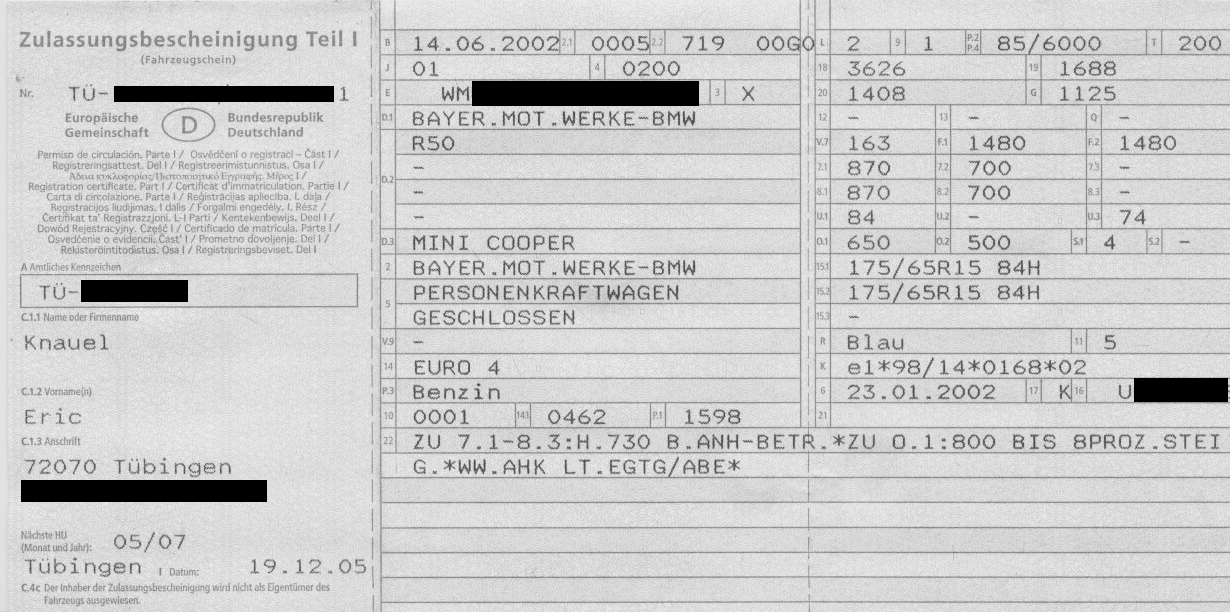
\includegraphics[width=\linewidth]{zusammengesetzte-daten/kfzschein-front}\\
      \medskip
      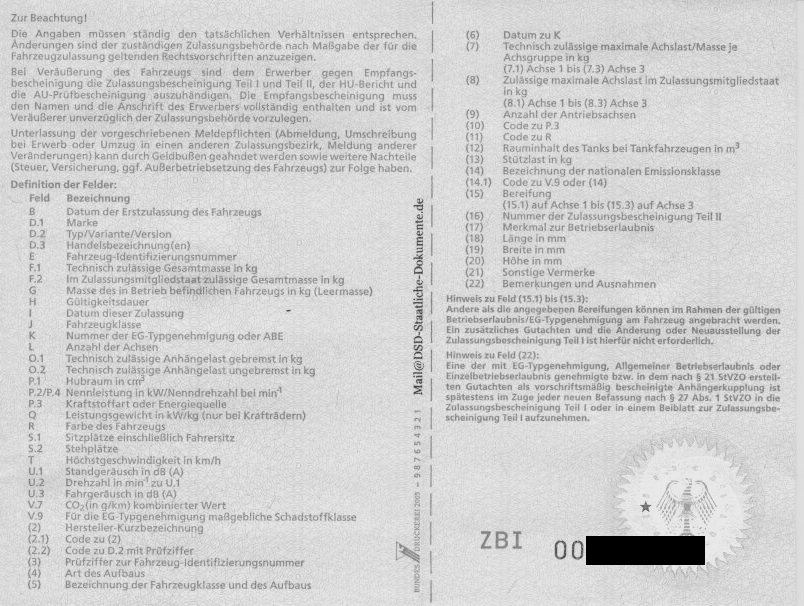
\includegraphics[width=\linewidth]{zusammengesetzte-daten/kfzschein-back}
      \caption{Vorder- und Rückseite eines Fahrzeugscheins}
      \label{fig:fahrzeugschein}
    \end{figure}
\end{aufgabe}

\begin{aufgabe}

  Schreibe für den Tübinger Stadtverkehr ein
  Programm, welches überprüft, ob ein Fahrzeug in den Umweltzonen fahren 
  darf.
  \begin{enumerate}
  \item Definiere einen Datentyp für Fahrzeuge. Dieser
    Datentyp soll den Typ, das Nummernschild und die Schadstoffklasse des
    Fahrzeuges beinhalten.
  \item Erstelle die Beispielfahrzeuge für die
    Fahrzeugtypen "<Stadtbus">, "<Reisebus">, "<Dieselauto">
    und "<Benzinauto">. Gehe davon aus, dass die Busse der
    Schadstoffklasse~2, das Dieselauto der Schadstoffklasse~3 und das
    Benzinauto der Schadstoffklasse~4 angehören.
  \item Schreibe eine Funktion \lstinline{fahrverbot?},
    welche überprüft, ob ein gegebenes Fahrzeug bei einer gegebenen
    Mindest-Schadstoffklasse noch fahren darf. Gestalte die Signatur
    so, dass er nur Mindest-Schadstoffklassen von 1 bis 4 akzeptiert.
  \item Die Mühlstraße in Tübingen ist in einer Richtung für
    alle Fahrzeuge außer Stadtbusse gesperrt. Schreibe eine Funktion
    \lstinline{sonderrecht?}, die überprüft, ob ein gegebenes Fahrzeug die
    Mühlstraße in der gesperrten Richtung befahren darf.  
  \item Der Stadtrat hat die Idee, den Tourismus
    dadurch anzukurbeln, dass Sonntags auch Reisebusse die Mühlstrasse in
    der gesperrten Richtunge befahren dürfen. Erweitere hierfür die
    Funktion \lstinline{sonderrecht?} um den Wochentag und lasse sonntags
    auch Reisebusse zu.
  \end{enumerate}
  Verwende beim Schreiben der Funktion die
  Konstruktionsanleitungen für Funktionen und für Fallunterscheidungen. 
  Schreibe Testfälle, die alle Möglichkeiten der   
  Fallunterscheidung abdecken.
  
\end{aufgabe}

\begin{aufgabe}

  Schreibe ein Programm für einen Paketdienst, das den Preis
  für ein Paket berechnet!
  \begin{enumerate}
    
  \item Schreibe eine Daten- und eine Record-Definition für
    \textit{Adressen}.  Zu einer Adresse gehören der Name, die Straße
    mit Hausnummer, die Postleitzahl, der Ort und das Land.
    
  \item Der Paketdienst verlangt einen Zuschlag für Sendungen, die
    international verschickt werden.  Schreibe eine Funktion
    \lstinline{international?}, die als Argument eine \textit{Adresse}
    bekommt und feststellt, ob die Adresse im Ausland liegt.

  \item Der Paketdienst hat einen Sondertarif für Sendungen, die
    innerhalb der gleichen Postleitzahl verschickt werden.  Schreibe
    eine Funktion \lstinline{same-zip-code?}, die als Argumente zwei
    \textit{Adressen} bekommt und feststellt, ob die Postleitzahlen
    und die Länder der beiden Adressen gleich sind.

  \item Ein Paket wird klassifiziert nach seinen Abmessungen.
    Schreibe eine Daten- und eine Record-Definition für
    \textit{Abmessungen}.  Abmessungen bestehen aus Länge, Breite und
    Höhe.

  \item Die Paketpreise richten sich nach der Größe des zu
    verschickenden Pakets.  Der Paketdienst verwendet die drei
    Größenklassen \textit{Small}, \textit{Medium} und \textit{Large},
    um die Kosten für das Paket zu berechnen.  Ausschlaggebendes
    Kriterium für die Paketgröße ist die Summe der längsten und der
    kürzesten Seite des Pakets.

    Schreibe eine Funktion
    \lstinline{add-longest-and-shortest-side}, die als Argument eine
    \textit{Abmessung} bekommt.  Der Rückgabewert von
    \lstinline{add-longest-and-shortest-side} soll die Summe der längsten
    und der kürzesten Seite der Abmessung sein.  Lagere die
    Teilprobleme in zwei Hilfsfunktionen aus: \lstinline{longest-side}
    und \lstinline{shortest-side}.

  \item Schreibe eine Daten- und eine Record-Definition für
    \textit{Pakete}.  Ein Paket hat eine Absender- und eine
    Empfängeradresse.  Benutze für die Adressen die bereits
    erstellte Record-Definition.  Außerdem hat ein Paket noch weitere
    Eigenschaften: Die Abmessungen (benutze dafür die bereits
    erstellte Record-Definition), das Gewicht, die Beförderungsdauer
    und eine Zusatz\-option Nachnahme.  Die Beförderungsdauer soll
    \emph{normal}, \emph{next-day} oder \emph{next-morning} sein.

  \item Schreibe eine Funktion \lstinline{parcel-size-class}, die
    als Argument ein \textit{Paket} bekommt und die Größenklasse
    zurückgibt.  Ausschlaggebend für die Paketgröße ist die Abmessung
    (siehe oben).  Folgende Tabelle enthält die Zuordnung von
    Paketgröße und Abmessung:

    \begin{center}
      \begin{tabular}{c|l}
        Paketgröße & Abmessung \\
        \hline
        S & 0--50 cm \\
        M & $>$50--100 cm \\
        L & $>$100 cm \\
      \end{tabular}
    \end{center}

  \item Schreibe eine Funktion \lstinline{calculate-base-postage},
    die als Argument ein \textit{Paket} bekommt und die
    Basis-Portokosten für dieses Paket berechnet.

    Lege dabei
    folgende Grundtariftabelle des Paketdienstes zugrunde:

    \begin{center}
      \begin{tabular}{c|ccc}
        & \multicolumn{3}{c}{Gewicht} \\
        Paketgröße & 0--5 kg & $>$5--10 kg & $>$10 kg \\
        \hline
        S & 3,00 & 6,00 & 9,00 \\
        M & 6,00 & 10,00 & 14,00 \\
        L & 9,00 & 15,00 & 21,00 \\
      \end{tabular}
    \end{center}

    

  \item Schreibe eine Funktion
    \lstinline{transportation-time-factor}, die als Argument ein
    \textit{Paket} bekommt und den Aufschlagsfaktor für die
    Beförderungsdauer zurückliefert.  Lege dabei folgende
    Aufschlagsfaktoren zugrunde:
    
    \begin{center}
      \begin{tabular}{c|ccc}
        & \multicolumn{3}{c}{Beförderungsdauer} \\
        Beförderungsdistanz & normal & next-day & next-morning \\
        \hline
        gleiche PLZ & -25\% & +0\% & +25\% \\
        Inland & +0\% & +50\% & +100\% \\
        Ausland & +100\% & +200\% & +300\% \\
      \end{tabular}
    \end{center}
    
  \item Schreibe eine Funktion
    \lstinline{cash-on-delivery-surcharge}, die als Argument ein
    \textit{Paket} bekommt und den Aufschlag für die Nachnahme
    zurückliefert.  Lege dabei folgende Aufschläge zugrunde:

    \begin{center}
      \begin{tabular}{c|c}
        Beförderungsdistanz & Nachnahmegebühr \\
        \hline
        Inland & +3,00 \\
        Ausland & +9,00 \\
      \end{tabular}
    \end{center}

  \item Schreibe eine Funktion \lstinline{calculate-postage}, die
    als Argument ein \textit{Paket} bekommt und die Portokosten
    berechnet.  Benutze dafür die bereits programmierten
    Lösungen der verschiedenen Teilprobleme.
    
  \end{enumerate}
  
\end{aufgabe}

%%% Local Variables: 
%%% mode: latex
%%% TeX-master: "i1"
%%% End: 
